% !TEX program = xelatex
\documentclass[12pt]{article}
\usepackage{ctex}
\usepackage{amsmath}
\usepackage{graphicx}
\usepackage{float}
\usepackage{booktabs}
\usepackage{geometry}
\geometry{a4paper, margin=2cm}

\title{\Huge \textbf{实验三 \quad正弦波振荡器}}
\author{专业：微电子科学与技术专业 \quad 学号：24308172 \quad 姓名：王钰铖}
\date{}

\begin{document}

\maketitle

\section*{一. 实验目的}
\begin{enumerate}
    \item 掌握LC反馈式正弦波振荡器的工作原理；
    \item 熟悉振荡器的幅度和相位起振条件；
    \item 了解电路各项参数（如反馈状态、负载特性等）对振荡器频率和振幅的影响；
    \item 掌握利用示波器与频谱仪测量及验证振荡频率和幅度特性的方法。
\end{enumerate}

\section*{二. 实验内容概要}

\vspace{1em}\noindent{\large \textbf{1. 实验原理概述：}}
\begin{itemize}
    \item \textbf{西勒（Seiler）振荡电路}：在电容三点式（Colpitts）基础上并在电感支路两端并联一个可调电容（本实验为受控制的变容二极管）所构成的改进型电路。其振荡频率近似为 $f \approx \frac{1}{2\pi\sqrt{L (C_p + C_v)}}$（$C_v$ 为变容管电容，$C_p$ 为回路等效并联分布电容）。由于调谐电容是并联接入的，在调节频率时，决定反馈深度的分压回路基本不受影响，因此可以在较宽频段内保持幅度的平稳输出。
    \item \textbf{克拉泼（Clapp）振荡电路}：在电容三点式电感支路中串联一个小容值电容（或变容二极管）构成的电路。回路串联等效总电容主要由该小电容决定，频率公式近似为 $f \approx \frac{1}{2\pi\sqrt{L C_v}}$。由于器件间隔离得更好，极大地减轻了晶体管结电容的影响，使得克拉泼电路频率稳定性极高。但由于串联连接，调谐频率升高时回路等效并联阻抗 $R_p$ 会发生断崖式下跌，容易引发高频幅值大幅衰落乃至停振。
    \item \textbf{晶体振荡器}：利用石英晶体极其陡峭的电抗频率特性（品质因数 $Q$ 极高）作为主选频网络的自激振荡器。极高的 $Q$ 值意味着极其微小的频移即可提供巨大的相位补偿，从而将整体振荡频率紧紧“死锁”在特定的标称值上。
\end{itemize}

\vspace{1em}\noindent{\large \textbf{2. 核心实验内容：}}
\begin{enumerate}
    \item[(1)] \textbf{西勒振荡电路实验}：测量稳态下不同变容二极管偏压对应的西勒电路振荡频率与幅值，绘制幅频特性，并认识并联调谐展现出的宽波段幅值平稳优势。
    \item[(2)] \textbf{克拉泼振荡电路实验}：将拓扑切换至串联调谐的克拉泼电路，测量全段电压响应，对比分析因阻抗下跌引起的高频率段幅值剧烈衰减现象。
    \item[(3)] \textbf{晶体振荡器实验}：使用示波器和频率表验证晶体振荡的高频率稳定度特性，通过调节静态偏置，探究工作点偏离对起振条件破坏和非线性畸变引发停振的物理过程。
\end{enumerate}

\section*{三. 具体实验}

\subsection*{任务一：西勒振荡电路实验}

根据实验要求接通电路，此时振荡电路配置为西勒振荡电路模式。逐步改变变容二极管两端的偏置电压，利用示波器测量记录对应的振荡频率 $f$ 和输出电压峰峰值 $V_{p-p}$，并记录在下表中。

\subsubsection*{1. 测试结果}

\begin{table}[H]
    \centering
    \makebox[\textwidth][c]{
        \begin{tabular}{|c|c|c|c|c|c|c|c|c|c|}
        \hline
        电压 (V) & 4 & 5 & 6 & 7 & 8 & 9 & 10 & 10.93 \\
        \hline
        振荡频率 $f$ (MHz) & 6.325 & 7.035 & 7.710 & 8.338 & 8.826 & 9.153 & 9.383 & 9.548 \\
        \hline
        输出电压 $V_{p-p}$ (V) & 1.319 & 1.591 & 1.767 & 1.930 & 1.952 & 2.052 & 2.110 & 2.100 \\
        \hline
        \end{tabular}
    }
    \caption{西勒振荡电路特性测试}
    \label{tab:seiler_results}
\end{table}

% （请在此处插入振荡频率与输出幅度的关系曲线图）
\begin{figure}[H]
\centering
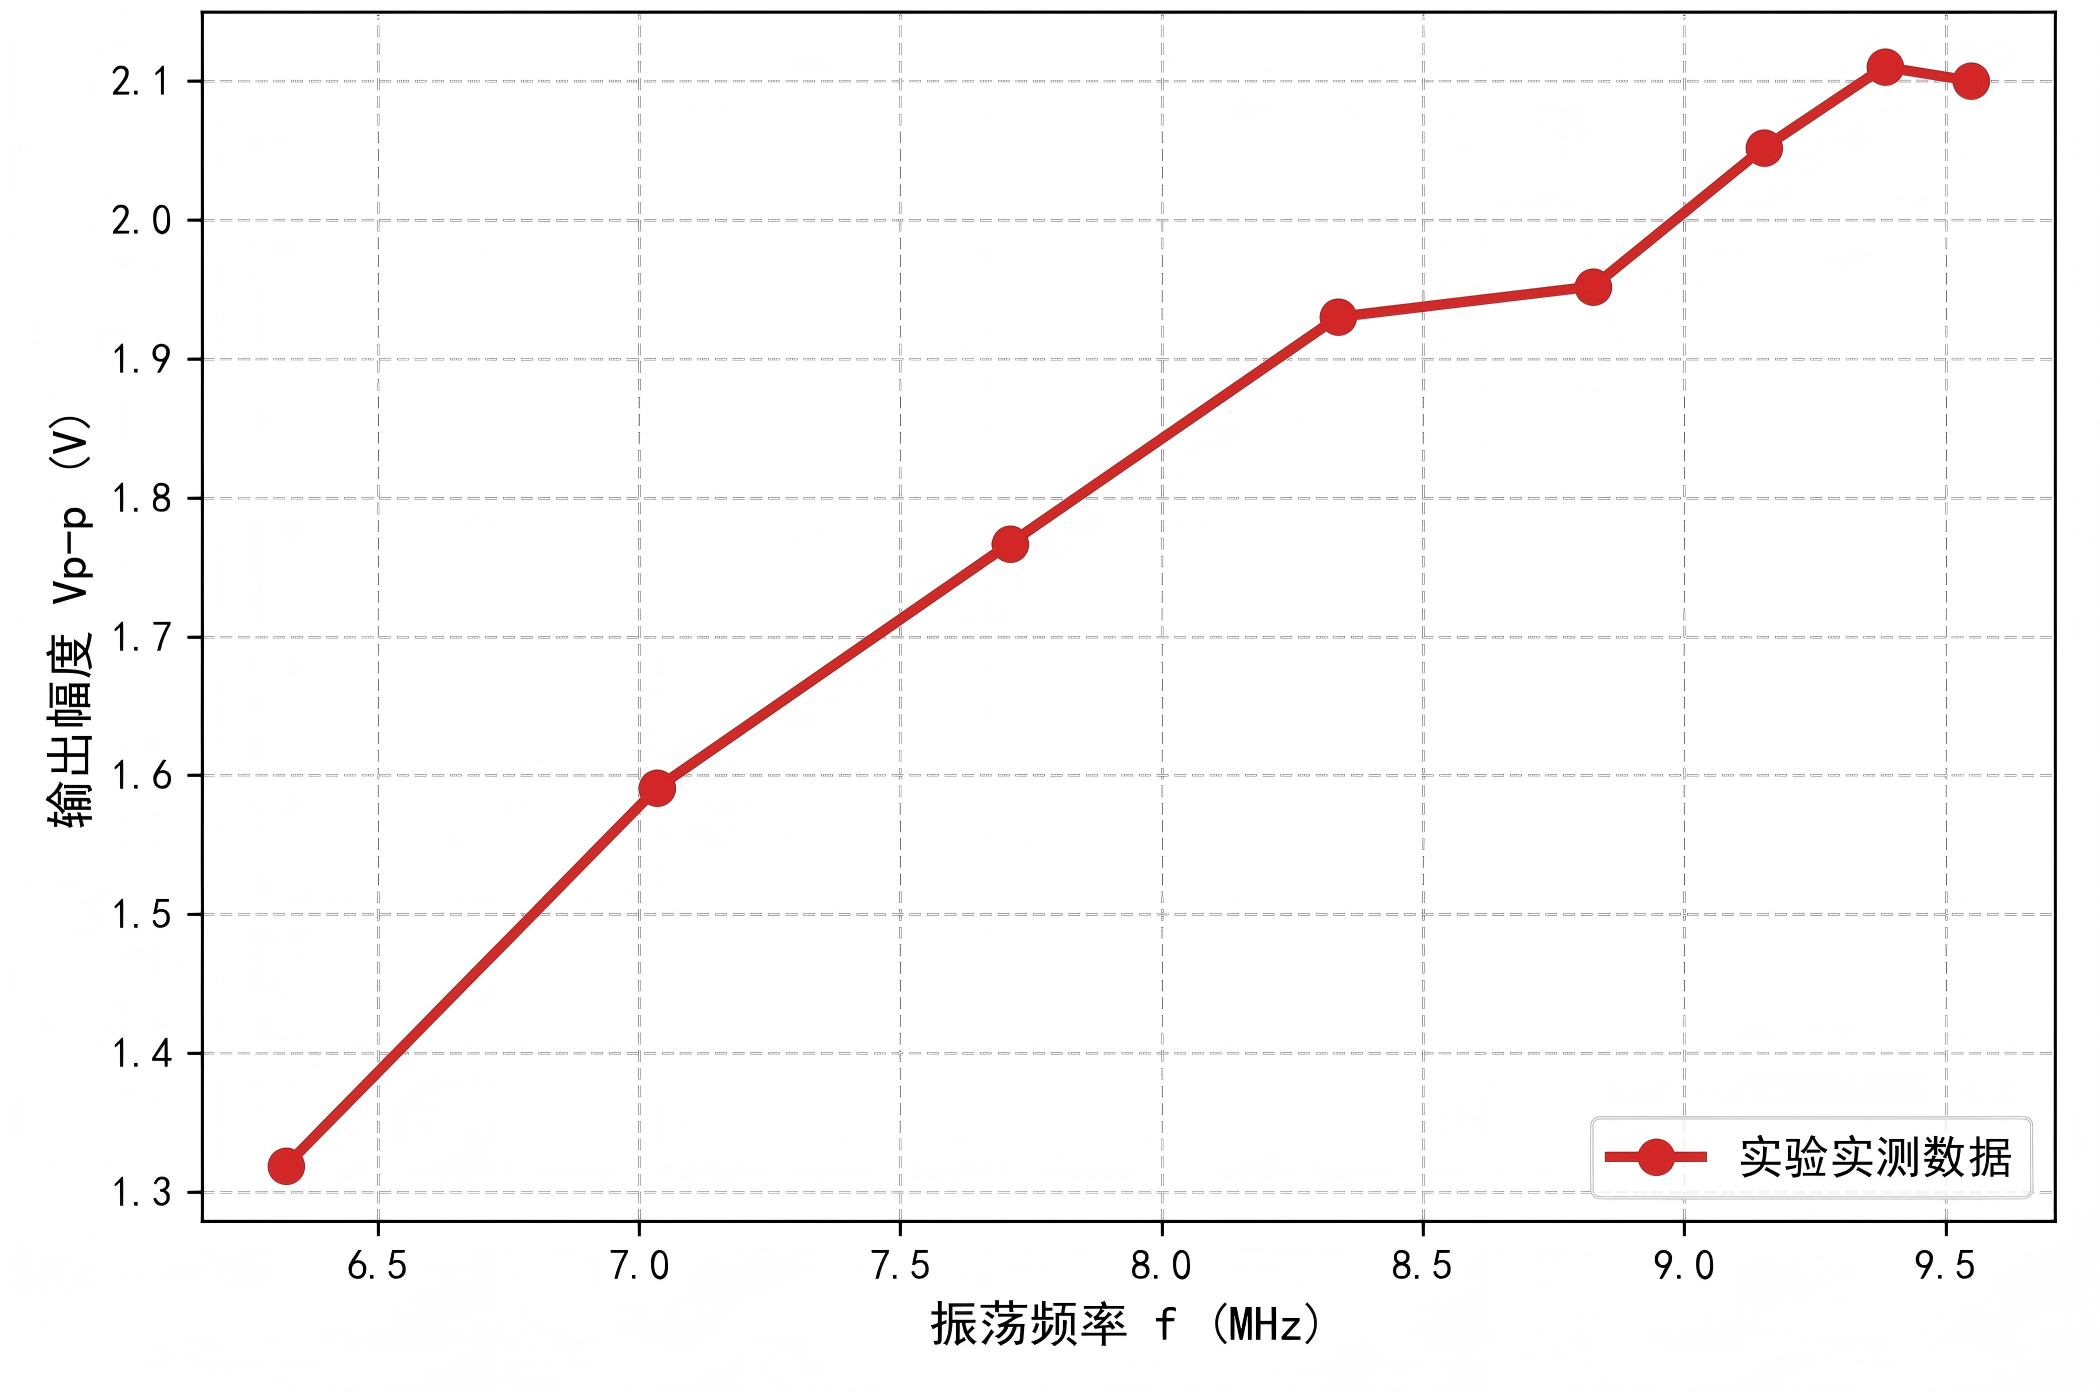
\includegraphics[width=0.8\textwidth]{西勒幅频特性.png}
\caption{西勒振荡电路振荡频率与输出幅度关系曲线}
\label{fig:seiler_curve}
\end{figure}

\subsubsection*{2. 结果分析}
\begin{itemize}
    \item \textbf{振荡频率与电容变化的关系：} 随着控制电压（反偏电压）的变化，变容二极管的电容表现出动态可调的特性。
    
    如测试数据所示，当控制偏压从 4V 增加到 10.93V 时，变容二极管的结电容逐渐减小。
    
    由于西勒振荡器回路的等效总电容主导着振荡频率，根据固有谐振频率公式 $f \approx \frac{1}{2\pi\sqrt{L C_{eq}}}$，等效电容的减小直接导致了振荡频率持续攀升。实测频率从 $6.325\text{MHz}$ 上升至 $9.548\text{MHz}$，验证了电压与振荡频率呈现正相关规律。
    \item \textbf{输出幅度与振荡频率的关系：} 随着振荡频率的逐渐升高，输出电压 $V_{p-p}$ 呈现出幅度显著上升并保持高位的变化趋势（由 $1.319\text{V}$ 上升至最高的 $2.110\text{V}$ 左右）。这是因为西勒电路中当频率升高时，反馈系数基本恒定，而晶体管集电极看到的谐振回路等效并联阻抗 $R_p$ 会随之增大。在两者作用下，放大器的环路增益 $AF$ 变大，从而振幅随之升高。
    \item \textbf{总结：} 由于其主反馈网络电容（分压反馈支路）未直接串入调谐支路中阻碍循环，因此在频段大范围调谐时，其反馈系数和晶体管看到的集电极等效并联阻抗的变化相比克拉泼电路更为平缓，使得振荡幅度在较宽的工作频段内都能维持相对平衡的稳定输出。
\end{itemize}

\subsection*{任务二：克拉泼振荡电路幅频特性的测量}

将开关 2K1 拨至“S”（往上拨），振荡电路转换为克拉泼电路。按照上述（1）的方法，通过改变电压调整回路电容，测出振荡频率和输出电压，并将测量结果记于表2-2中。

\subsubsection*{1. 测试结果}

\begin{table}[H]
    \centering
    \makebox[\textwidth][c]{
        \begin{tabular}{|c|c|c|c|c|c|c|c|c|c|c|c|}
        \hline
        电压 (V) & 0 & 0.5 & 1 & 1.5 & 2 & 2.5 & 3 & 3.5 & 4 & 4.5 & 5 \\
        \hline
        振荡频率 $f$ (MHz) & 7.863 & 8.063 & 8.286 & 8.512 & 8.730 & 8.999 & 9.311 & 9.692 & 10.100 & 10.640 & 11.270 \\
        \hline
        输出电压 $V_{p-p}$ (V) & 2.120 & 2.070 & 2.032 & 2.002 & 1.984 & 2.002 & 1.876 & 1.827 & 1.775 & 1.723 & 1.601 \\
        \hline
        \end{tabular}
    }
    \caption{克拉泼振荡电路特性测试}
    \label{tab:clapp_results}
\end{table}

\begin{figure}[H]
\centering
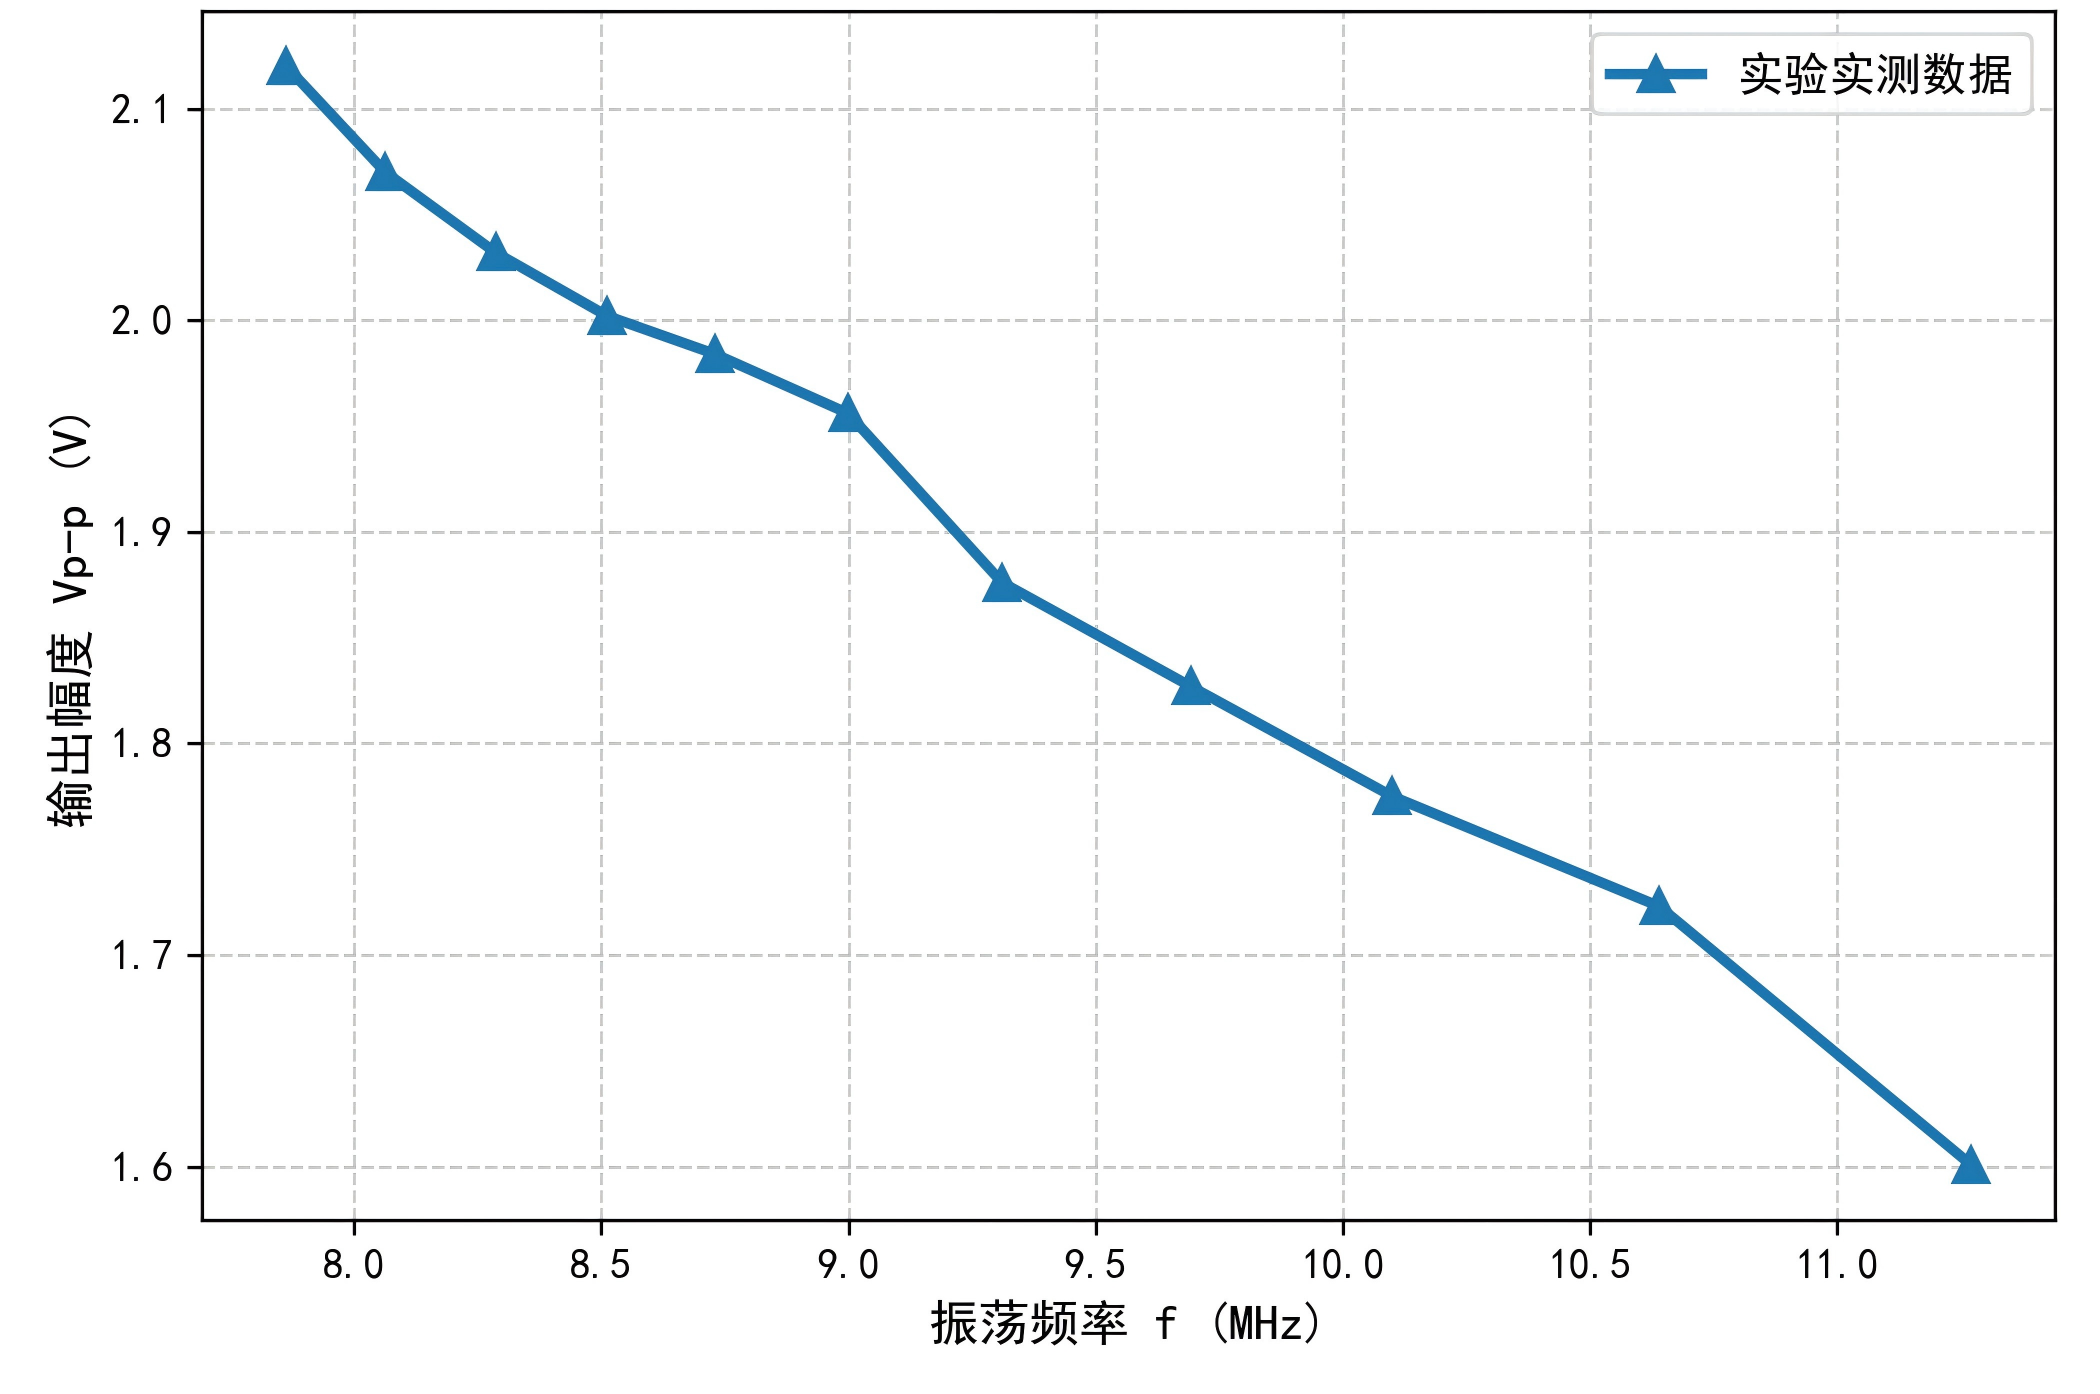
\includegraphics[width=0.8\textwidth]{克拉泼幅频特性.png}
\caption{克拉泼振荡电路振荡频率与输出幅度关系曲线}
\label{fig:clapp_curve}
\end{figure}

\subsubsection*{2. 结果分析}
\begin{itemize}
    \item \textbf{频率与电容变化规律对比：} 将电路切换至克拉泼振荡器后，同样调节反偏电压（0~5V），频率随偏压增大而单调升高（从 $7.863\text{MHz}$ 上升至 $11.270\text{MHz}$）。
    
    克拉泼电路的特点在于调谐主电容（本实验中为变容二极管主导的等效电容支路）与两个具有较大容数值的反馈电容呈串联结构，这种隔离作用使得等效总电容很大程度上只取决于主调谐电容。
    
    因此，调节变容二极管电容对振荡频率的控制极为灵敏且频段更宽，频率稳定度也相应更高。
    \item \textbf{输出幅度变化规律：} 克拉泼振荡电路中反映出了典型的非线性衰减现象。如数据及曲线所示，随着振荡频率的提高（即电路电容减小），输出振幅 $V_{p-p}$ 出现了显著的主动下降（由 $2.120\text{V}$ 一路跌落至 $1.601\text{V}$ 甚至更低）。这是因为克拉泼电路中调谐主电容与电感呈串联状态接入，当振荡频率攀升时会导致整个晶体管谐振回路等效并联阻抗 $R_p$ 变得非常小（近似与频率的三次方成反比）。这种阻抗的跌落使得实际闭环增益 $AF$ 大幅减弱，如果频率进一步被调高直到 $AF < 1$ 时，就不再满足起振的幅度平衡条件，从而完全停振。
\end{itemize}

\subsection*{任务三：晶体振荡器实验}

具体实验步骤如下：
\begin{enumerate}
    \item[(1)] 用铆孔线将 2P3 与 2P4 相连，将双通道示波器探头接至 2TP5 端以观察晶体振荡器建立的波形。若未能观测到稳态的正弦波形，需要调整 2W3 电位器直至起振。随后，利用频率计（或示波器内置测量功能）测量输出端 2P5 的实际频率，校对是否与所加晶体的标称标定频率（9.0MHz）一致。
    \item[(2)] 保持示波器监测 2TP5 端，频率计监视 2P5 输出端。缓慢调节 2W3 电位器以改变晶体管静态工作点，仔细观察振荡波形的动态失真演变乃至停振状态出现；同时高度注意在调平全过程中，由于工作点变化是否会牵引影响拉动振荡频率发生偏移。
\end{enumerate}

\subsubsection*{1. 测试结果}

\begin{figure}[H]
\centering

\includegraphics[width=0.8\textwidth]{频率计测量输出频率.jpg}
\caption{频率计测量输出端频率}
\label{fig:clapp_curve}
\end{figure}

\begin{figure}[H]
    \centering
    \begin{minipage}[t]{0.32\textwidth}
        \centering
        \includegraphics[width=\textwidth]{晶体振荡器.png}
        \caption{正常稳态振荡波形}
    \end{minipage}
    \hfill
    \begin{minipage}[t]{0.32\textwidth}
        \centering
        \includegraphics[width=\textwidth]{晶体振荡器（略有失真）.png}
        \caption{失真波形}
    \end{minipage}
    \hfill
    \begin{minipage}[t]{0.32\textwidth}
        \centering
        \includegraphics[width=\textwidth]{晶体振荡器（停振）.png}
        \caption{调节2W3偏置后的停振状态}
    \end{minipage}
    \vspace{0.5em}
    \label{fig:xtal_osc_pics}
\end{figure}


\subsubsection*{2. 结果分析}
\begin{itemize}
    \item \textbf{晶体谐振特性与高频稳定性：} 在正常起振状态下，由测试频率可知输出频率锁定在 $9.0\text{MHz}$ 附近极窄频段内。石英晶体振荡器能够提供远超级别 LC 回路频移抗性。
    石英晶片具有优异的压电效应和相频特性曲线梯度，电路周遭环境杂散感抗变化引起的剧烈相位抖动，石英晶体会提供极度微小的频移来补齐 $2n\pi$ 的相频平衡需求去锁定频率。
    \item \textbf{静态工作点变化对起振与波形条件的影响规律：} 实验步骤(2)通过调节 2W3，实质上是在调整晶体管的偏置状态。
    
    随着直流工作点发生偏移，放大晶体管极容易脱离原有的理想放大或甲乙类浅自激状态滑入严重饱和或截止区域；反馈增益倍数由于集电极静态电流被挤压而大幅度滑坡。
    
    当小信号净跨导以及回路增益剧烈衰减致破坏起振的幅度平衡核心条件 $AF \ge 1$ 闭环后，系统从明显出现顶/底削平的非线性失真快速演变为幅面骤缩乃至完全跌入死区的停寂态（停振）。
    
    当直流工作点还存在可以振荡的范围内，有摆波存留，其振荡信号频段依旧可控在 $9.0\text{MHz}$ ，展现石英晶体的优越物理特性。
\end{itemize}

\section*{四. 总结}

% 【在此处填入今日实验的具体总结和感想，以下给出一部分参考框架可直接采纳或修改】

本次《正弦波振荡器》实验，让我深刻学习了非线性电路中“自激振荡”的内容。相比于第一节实验中需要外部输入信号源的调制放大器，本次振荡器实验是纯粹依仗内部正反馈机制与晶体管的非线性实现能量转换的过程。

通过调节参数，电路从“不起振”跃迁到“幅度受限的完全稳态振荡”，我们观察到波形与数据的对应。实验直接验证了LC选频网络的调谐参数会控制频率，而偏置和反馈回路的参数决定了振荡幅度及起振难度。

由于高频状态下元器件的高频微变电容（如晶体管结电容）无法再作为理想器件忽略，实验测出的真实震荡频率也会相比简单理论手算的有所偏差。针对这些特性的系统测试，启发我在未来的模拟电路设计中留有调整余量。

\end{document}
